% This is LLNCS.DEM the demonstration file of
% the LaTeX macro package from Springer-Verlag
% for Lecture Notes in Computer Science,
% version 2.2 for LaTeX2e
%
\documentclass[runningheads]{llncs}
%
%\usepackage{makeidx}  % allows for indexgeneration
\usepackage{graphicx}
\usepackage{times}
\usepackage{rotate}
\usepackage{lscape}

%% MES PACKAGES/COMMANDES

\usepackage{amsmath}
\usepackage{amsfonts}
\usepackage{amssymb}
\usepackage{multicol}
\usepackage{mathenv}
\usepackage[utf8]{inputenc}

\usepackage[french]{babel}
\selectlanguage{french}

\usepackage{color}
%\usepackage{hyperref}
%\hypersetup{pdfborder={0 0 0}, colorlinks=true, urlcolor=blue, linkcolor = darkred}
\usepackage{verbatim}
\usepackage{moreverb}

\definecolor{darkred}{rgb}{0.85,0,0}
\definecolor{darkblue}{rgb}{0,0,0.7}
\definecolor{darkgreen}{rgb}{0,0.6,0}
\definecolor{darko}{rgb}{0.93,0.43,0}
\definecolor{maintitle}{rgb}{0.66,0,0.22}
\definecolor{title}{rgb}{0,0.5,0.5}

\newcommand{\maintitlecolor}[1]{\textcolor{maintitle}{#1}}
\newcommand{\titre}[1]{\textcolor{title}{#1}}
\newcommand{\tsect}[1]{\titre{\section{#1}}}
\newcommand{\tssect}[1]{\titre{\subsection{#1}}}
\newcommand{\tsssect}[1]{\titre{\subsubsection{#1}}}
\newcommand{\vect}[1]{\overrightarrow{#1}}
\newcommand{\dred}[1]{\textcolor{darkred}{\textbf{#1}}}
\newcommand{\dgre}[1]{\textcolor{darkgreen}{\textbf{#1}}}
\newcommand{\dblu}[1]{\textcolor{darkblue}{\textbf{#1}}}
\newcommand{\dora}[1]{\textcolor{darko}{\textbf{#1}}}
\newcommand{\gre}[1]{\textcolor{darkgreen}{#1}}
\newcommand{\blu}[1]{\textcolor{darkblue}{#1}}
\newcommand{\ora}[1]{\textcolor{darko}{#1}}
\newcommand{\red}[1]{\textcolor{darkred}{#1}}
\newcommand{\ceil}[1]{\left\lceil #1 \right\rceil}
\newcommand{\cdil}[1]{\left\lfloor #1 \right\rfloor}
\newcommand{\term}[1]{\textit{\textcolor{maintitle}{#1}}}
\newcommand{\image}[1]{\includegraphics{#1}}
\newcommand{\imageR}[2]{\includegraphics[width=#2px]{#1}}
\newcommand{\imageRT}[2]{\includegraphics[height=#2px]{#1}}
\newcommand{\img}[1]{\begin{center}\includegraphics[width=400px]{#1}\end{center}}
\newcommand{\imag}[1]{\begin{center}\includegraphics{#1}\end{center}}
\newcommand{\imgR}[2]{\begin{center}\includegraphics[width=#2px]{#1}\end{center}}
\newcommand{\imgRT}[2]{\begin{center}\includegraphics[height=#2px]{#1}\end{center}}
\newcommand{\point}[2]{\item \ora{\underline{#1}} : \textit{#2}}
\newcommand{\bfp}[2]{\item \textbf{#1} : \textit{#2}}
\newcommand{\sumparam}[3]{\sideset{}{_{#1}^{#2}}\sum{#3}}
\newcommand{\sumin}[3]{\sideset{}{_{i=#1}^{#2}}\sum{#3}}
\newcommand{\sumkn}[3]{\sideset{}{_{k=#1}^{#2}}\sum{#3}}
\newcommand{\intin}[3]{\sideset{}{_{#1}^{#2}}\int{#3}}
\newcommand{\stitre}[1]{\noindent\textbf{\underline{#1}} \\}
\newcommand{\R}{\mathbb{R}}
\newcommand{\Z}{\mathbb{Z}}
\newcommand{\N}{\mathbb{N}}
\newcommand{\ualpha}{\vect{u_\alpha}}
\newcommand{\valpha}{\vect{v_\alpha}}
\newcommand{\palpha}{\vect{\Psi_\alpha}}
\newcommand{\npcomp}{\term{$\mathcal{NP}$-complet}}
\newcommand{\npcompl}{\term{$\mathcal{NP}$-complet} }

%% FIN MES PACKAGES/COMMANDES

%% DEBUT DU DOCUMENT
%\usepackage{rotate}
%\usepackage{lscape}
%\usepackage{subfigure}

%\usepackage[draft]{fixme}
\begin{document}

\frontmatter          % for the preliminaries
\pagestyle{headings}  % switches on printing of running heads
\mainmatter              % start of the contributions
\title{The Mythical Man-Month : \\
Chapitre 7 : Why Did the Tower of Babel Fail ? \\
Chapitre 8 : Calling the Shot\\}
%
\titlerunning{Why Did the Tower of Babel Fail ? - Calling the Shot}
% abbreviated title (for running head)
%                                     also used for the TOC unless
%                                     \toctitle is used
%
\author{DUBUC XAVIER}
%
\authorrunning{DUBUC XAVIER - 1e ann\'ee du master en sciences informatiques} 

\tocauthor{Tom Mens (Universit\'e de Mons)}

\institute{Facult\'e des Sciences, Universit\'e de Mons\\
Av. du champ de Mars 6, 7000 Mons, Belgium\\
\email{XAVIER.DUBUC@student.umons.ac.be}
%VOUS POUVEZ UTILISER UN AUTRE ADRESSE MAIL QUE CELUI DE L'UMH SI VOUS LE PREFERIEZ
}
\maketitle              % typeset the title of the contribution

%UTILISEZ LE SUIVANT DANS LE CAS D'UN CHAPITRE DU LIVRE:
\begin{abstract}
Ce rapport est rendu dans le cadre du cours de ``Gestion de Projets Logiciels" (dispens\'e par Monsieur \emph{Tom Mens} en ann\'ee acad\'emique 2010-2011). Le but de ce rapport est de r\'esumer, d'analyser, et de se former une appr\'eciation personnelle d'un chapitre du livre\cite{Brooks1995}. Il s'agit des chapitres 7 et 8 intitul\'es respectivement \textit{Why Did the Tower of Babel 
Fail ?} et \textit{Calling the Shot}.
\end{abstract}


%%%%%%%%%%%%%%%%%%%%%%%%%%%%%%%%%%%%%%%%%%%%%%%%
%%%%%%%%%%%%%%%%%%%%%%%%%%%%%%%%%%%%%%%%%%%%%%%%
\newpage
\section{R\'esum\'e du chapitre}\label{sec:resume}

\subsection{Chapitre 7 : Why Did the Tower of Babel Fail ?}

Ce chapitre traite des essentiels que doit posséder un projet afin qu'il soit mener à son terme et ce, dans les meilleurs délais 
et avec la meilleure qualité. Les 2 éléments les plus importants à gérer dans un projet sont l'\textbf{organisation} et la 
\textbf{communication}. \\

C'est ce dernier point qui a fait défaut à la construction de la tour de Babel car le Seigneur est
intervenu pour que la langue unique ne soit plus d'actualité, les hommes ne pouvant plus se \textbf{comprendre} (\red{mauvaise 
communication}), ils ne pouvaient plus s'\textbf{organiser} (\red{mauvaise organisation}). La mauvaise communication peut aussi
mener à des groupes de personnes isolées, personnes préférant éviter les conflits avec les autres groupes (jalousie, disputes, 
...). \\

\noindent\textbf{La communication dans les grands projets de programmation} \\
De nos jours, les problèmes de calendrier, les incompatibilités fonctionnelles et les bugs de système surgissent à cause du fait
qu'une partie d'un projet ne sait pas ce que fait l'(les) autre(s) partie(s). Afin d'éviter ces désagréments, les différentes
parties d'un projet doivent avoir une \gre{bonne communication} et ce, de toutes les manières possibles :
\begin{itemize}
\item \textbf{de manière informelle} via un bon service téléphonique et une définition claire des dépendances entre groupes,
\item \textbf{via des réunions} (précieuses) de projet régulières où les équipes présentent des briefings techniques,
\item en utilisant un \textbf{project workbook} (littéralement "classeur de projet") que l'on initialise dès le début du projet.\\
\end{itemize}

\noindent\textbf{Project Workbook}\\
Ce \textit{project workbook (\textbf{PW})}, est un document à part régissant la structure des documents que le projet va fournir
quoi qu'il arrive. Chacun de ces documents doit faire partie de cette structure, cela inclut :
\begin{itemize}
\item les objectifs,
\item les spécifications externes,
\item les spécifications internes,
\item les spécifications de l'interface,
\item les standards techniques,
\item les mémos administratifs.
\end{itemize}
\noindent $\rightarrow$ \textbf{Pourquoi utiliser un PW ?}
\begin{enumerate}
\item La première raison est que la prose technique est quasi immortelle, si on examine la généalogie d'un tel document, on peut
non seulement retracer les idées mais aussi une grande partie des phrases du premier mémo qui propose le produit ou explique le
premier design. Vu que les documents suivants vont se baser sur le document courrant, il est très important d'avoir une bonne
structure.
\item La seconde est qu'il permet le contrôle de la distribution de l'information. L'idée n'est pas de restreindre l'information
mais d'assurer que l'information pertinante parvienne à toutes les personnes qui en ont besoin. Pour ce faire, on numérote chaque
mémo de manière à ce que des listes ordonnées de titres soient disponibles et que chaque travailleur puisse voir s'il a ce qu'il 
veut. L'organisation du classeur va bien au delà de ça pour établir un structure d'arbre des mémorandums, structure qui permet aux 
listes de distribution d'être maintenues par un sous-arbre si c'est désirable. \\
\end{enumerate}

\noindent\textbf{En pratique}\\
Il faut savoir que le problème du mémo technique n'est pas linéaire avec la taille du projet, ainsi, par exemple, pour un projet
regroupant 1000 personnes (qui sont inévitablement dispersées dans des endroits géographiques différents) le besoin du \textbf{PW}
est grand tout comme la taille de celui-ci. Il faut donc trouver un bon moyen de le tenir à jour. Par exemple, pour le projet de
l'OS/360, ils disposaient d'un système d'édition de texte dirigé par un ordinateur dont ils étaient content mais après 6 mois de 
projet le \textbf{PW} faisait environ 1.524m de large ! \textit{(Ils avaient 100 bureaux et donc 100 copies du \textbf{PW} et, 
s'il les empilait, la pile dépassait le toit du Manhattan's Time-Life Building)} De plus, les mises à jour faisaient environ 5 
centimètres, donc environ 150 pages à insérer à chaque fois dans le \textbf{PW} $\Rightarrow$ l'entretien du \textbf{PW} prenait
un temps conséquent.

\begin{figure}
\begin{center}
  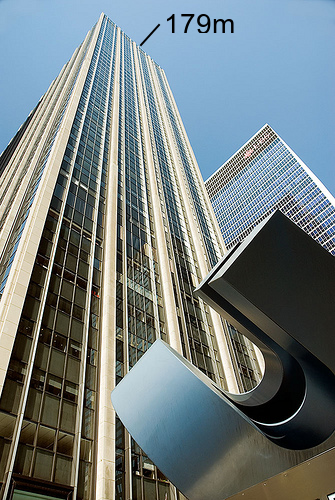
\includegraphics[width=150px]{img1.png}
  \caption{Manhattan's Time-Life Building.}
\end{center}
\end{figure}

N'ayant pas le choix, ils ont changé leur fonctionnement et ont opté pour les \textbf{microfiches}, changement qui a sauvé 1 
million de dollars (même en tenant compte du prix des lecteurs de microfiches (un/bureau)), le PW a diminué de $0.0849 m^3$ à 
$0.00429 m^3$ et les mises à jour apparaissaient par morceau de centaines de pages, réduisant par 100 le problème d'insertion.
Néanmoins ces microfiches ont leurs inconvénients, elles ne peuvent par exemple pas être marquées, surlignées, ... \\

\noindent\textbf{De nos jours (90's)}\\
Avec la technologie de systèmes de nos jours, le livre suggère que la meilleure technique de choix est de garder le classeur sur 
les fichiers à accès direct, marqué par des barres de changements et des dates de révision. Chaque utilisateur le consulterait 
depuis un terminal d'affichage (les machines à écrire sont trop lentes). Un résumé des changements, préparé chaque jour, serait 
stocké de manière LIFO dans un point d'accès fixé. Le programmeur lirait probablement ceci quotidiennement, mais s'il manque un 
jour il n'aura qu'à lire un peu plus le jour de son retour. Pendant qu'il lit le résumé des changements, il peut s'interrompre 
pour consulter le texte modifié.\\

\noindent\textbf{L'organisation dans les grands projets de programmation} \\
Projet : $\red{n}$ travailleurs $\Rightarrow$ $\red{\frac{(n^2-n)}{2}}$ interfaces de la communication \\ 
\indent $\qquad\qquad\qquad\quad\ \Rightarrow $ $\red{2^n}$ équipes potentielles à coordonner.\\
Le but de l'organisation est de réduire \textbf{le nombre de communications} et \textbf{de coordinations nécessaires}; ainsi 
l'organisation est une attaque radicale contre les problèmes de communication traités précédemment. Pour éviter les 
communications, il est de bon ton d'utiliser les mécanismes de management bien connus que sont \textbf{la division du travail} et
\textbf{la spécification fonctionnelle}, l'utilisation de ces 2 mécanismes impliquent que la structure de l'entreprise devient un
arbre (cf. le principe de Fayol disant qu'un employé ne peut obéir à 2 chefs différents). Dans une telle structure, chaque sous-
arbre doit contenir 6 essentiels pour être fonctionnel :
\begin{enumerate}
\item une mission,
\item un \blu{producteur},
\item un \blu{directeur ou architecte technique},
\item un calendrier,
\item une division du travail,
\item des définitions d'interface entre les parties.
\end{enumerate}
Toutes ces choses sont évidentes et conventionnelles exceptés la distinction entre le \blu{producteur} et le \blu{directeur 
technique}.\\

\noindent\textbf{Le rôle du producteur}\\
Il rassemble l'équipe, divise le travail, établit le calendrier (et s'assure qu'il est respecté) et acquiert les ressources 
nécéssaires. Cela signifie qu'une majeure partie de son rôle consiste en \textbf{communications en dehors de son équipe} 
\textit{(envers les instances supérieures ou avec des collègues du même niveau que lui)}. Il établit le modèle de communication et 
de rapports à l'intérieur de l'équipe.\\

\noindent\textbf{Le rôle du directeur technique}\\
Il conçoit le design à construire, identifie les sous-parties, spécifie à quoi ça va ressembler vu de l'extérieur et esquisse la 
structure interne. Il fournit l'unité et l'intégrité conceptuelle à tout le design; il sert donc comme limite à la complexité du 
système. Quand des problèmes techniques individuels surgissent, il invente des solutions à ceux-ci ou il change le design du 
système comme il est requis. Ses \textbf{communications sont principalement "intra-équipe"} et son travail est presque 
complètement technique.\\

\noindent\textbf{Relation producteur-directeur technique}\\
Maintenant qu'il est clair que les 2 rôles demandent des talents différents, il y a 3 situations possibles :
\begin{enumerate}
\item \textbf{Le producteur et le directeur technique sont la même personne}, c'est réalisable sur de très petites équipes de 
l'ordre de 3 à 6 programmeurs et pas sur de plus grand projets, pour 2 raisons :
	\begin{enumerate}
	\item la personne la meilleure en management ET en technique est rarement trouvée,
	\item difficile pour le producteur de déléguer assez de ses fonctions pour s'occuper de son rôle de directeur technique et, 
	dans l'autre sens, c'est impossible pour le directeur technique de déléguer sans compromettre l'intégrité conceptuelle du 
	projet
	\end{enumerate}
\item \textbf{Le producteur est le boss et le directeur technique est son bras droit}, la difficulté étant d'établir l'autorité du
directeur technique à prendre des décisions sans impact tel sur son temps qu'il serait placé dans la chaine de commande du 
management. Le producteur se doit de proclamer l'autorité du directeur technique et ces 2 hommes doivent avoir la même vue sur la 
philosophie technique fondamentale et ils doivent discuter sur les questions techniques de manière privée avant qu'elles ne 
deviennent opportunes. Cette structure peut être organisée pour être efficiente mais est, hélas, rarement essayée en pratique.
\item \textbf{Le directeur technique est le boss et le producteur est son bras droit}, Le producteur est au petit soin du 
directeur technique, le déstresse, le détend etc de manière à ce qu'il n'ait qu'à se concentrer sur l'ingénierie. Le producteur 
proclame également son autorité suprême et dans tout ce qui est publique c'est lui qui sera crédité. Cet arrangement peut 
également être organisé de manière à fonctionner de manière effective, mais le livre suspecte que cet arrangement est mieux adapté
pour les petites équipes.
\end{enumerate}
Brooks pense que le \textbf{producteur comme boss} est l'arrangement le plus fiable pour les plus gros sous-arbres d'un vraiment 
gros projet. \\

\textbf{En conclusion}, la tour de Babel était peut-être le premier fiasco de l'ingénieurie mais ce n'était pas le dernier. La 
communication et ses conséquences ainsi que l'organisation sont critiques pour la réussite. Les techniques de communication et 
d'organisation demandent du manager plus de pensées et autant de compétences d'expérience que la technologie du logiciel lui-même.

\newpage
\subsection{Calling the Shot}

Ce chapitre traite de l'estimation du temps et des efforts à fournir pour un projet de programmation. Tout d'abord il faut savoir 
qu'il ne suffit pas d'estimer la portion de code mais qu'il faut également tenir compte du planning, de la documentation, des 
tests (des composants et du système), de l'intégration du système et les temps de formation. Ensuite, les données que l'on 
trouvera pour un petit projet ne pourront pas être utilisée pour les plus grand projets et inversément (par exemple un projet 
contenant en moyenne 3200 mots (langage assembleur) ayant demandé 178 heures à un programmeur donne une productivité de 35 800 
mots par an, tandis qu'un projet 2 fois plus petit prendra environ le quart du temps et donne une productivité de 80 000 mots par 
an. Ces nombres nous suggèrent que l'effort augmente comme une puissance de la taille. Des études ont montré que l'on pouvait 
estimer l'effort comme suit : \begin{center}effort $=$ (constante) $\times (\text{nombre d'instructions})^{1.5}$\end{center}

D'autres études ont été faites sur la productivité d'un programmeur, en voici un court aperçu des plus éclairantes d'entre elles :
\begin{enumerate}
\item \textbf{les données de Portman}, elles mettent en évidence le fait que seulement la moitié du temps que possède le 
programmeur est vraiment utilisé à programmer et à débugger, l'autre moitié contient le temps d'arrêt des machines, les petits 
jobs de plus haute priorité non lié au projet, les réunions, la paperasserie, le business de l'entreprise, la maladie, le temps 
personnel, ... \\
$\Rightarrow$ Les estimations font une hypothèse irréaliste à propos du nombre d'heures de travail technique par 
personne/an.
\item \textbf{les données de Aron}, elles mettent en évidence le fait que plus il y a d'interactions entre les programmeurs, plus 
la productivité diminue.
\item \textbf{les données de Harr}, elles présentent des données concernant 4 programmes de taille similaire différents uniquement
au niveau de la taille des groupes de travail, le temps pris et le nombre de modules. On constate dès lors que ces programmes 
donnent des productivités complètement différentes et \textbf{Brooks} pense que ces programmes diffèrent également sur la 
complexité des problèmes.
\item \textbf{les données de l'OS/360}, elles confirment les données de \textbf{Harr}. \\
$\Rightarrow$ Les données de \textbf{Harr}, d'\textbf{Aron} et de l'\textbf{OS/360} confirment toutes des différences frappantes 
dans la productivité reliées à la complexité et à la difficulté de la tâche elle-même. 
\item \textbf{les données de Corbató}, ces données concernent le système d'exploitation MULTICS (entre 1 million et 2 millions de 
mots, langage de plus haut niveau que l'assembleur), elles suggèrent 2 importantes conclusions :
	\begin{enumerate}
	\item La productivité semble être constante en terme de "statements élémentaires", une conclusion qui est raisonable en terme 
	de la pensée qu'un statement recquiert et les erreurs qu'elle peut comporter.
	\item La productivité de programmation peut être multipliée par 5 lorsqu'un langage de programmation de haut niveau approprié 
	est utilisé.
	\end{enumerate}
\end{enumerate}

%%%%%%%%%%%%%%%%%%%%%%%%%%%%%%%%%%%%%%%%%%%%%%%%
%%%%%%%%%%%%%%%%%%%%%%%%%%%%%%%%%%%%%%%%%%%%%%%%
\newpage
\section{Analyse et appr\'eciation personnelle du chapitre}\label{sec:analyse}

\subsection{Analyse globale}

La première chose qui me choque dans ce livre et qui ne m'a pas trop plu, c'est l'utilisation de la première personne pour 
traiter les sujets. N'étant pas très friant de ce type de littérature à la base, cela ne m'a pas aidé. De plus, je trouve que pour
traiter des sujets scientifiques comme dans ce livre, la troisième personne est plus appropriée, elle assure (ou du moins donne 
l'illusion) l'objectivité de l'auteur. \\

Ensuite, l'anglais utilisé est assez imagé et soutenu ce qui n'est pas évident pour nous, pauvres francophones dont les 
connaissances en anglais sont assez limitées (bien que je me considère assez bon en anglais). La compréhension du texte en est dès 
lors très altérée (il se peut d'ailleurs que certains passages aient été mal compris) et la lecture, fastidieuse, devient vite une 
corvée. \\

Au final, le fait que les chiffres donnés concernent des vieux projets, on ne comprend pas trop ce que représente un "mot" ou un
"statement" en langage assembleur, de plus les ordinateurs n'étaient pas encore monnaie courrante à cette époque, ce qui fait que
certains mécanismes ne sont plus d'actualités (comme les microfiches et les terminaux d'affichage dans le chapitre 7 par exemple).

\subsection{Chapitre 7 : Why Did the Tower of Babel Fail ?}

J'ai trouvé le titre accrocheur de prime abord mais ensuite je me suis assez ennuyé à la lecture de ces pages. En effet, la 
majeure partie des éléments développés ont été vu dans le cours de \textit{«Management»} (dispensé par monsieur Labie) de l'année 
passée, ce n'était donc, pour la plupart, que du rappel. En dehors de ça, le management étant un point important des entreprises 
de nos jours et celui-ci n'ayant pas changé depuis les années 70, ce chapitre est pertinent et encore d'actualité. (bien sûr les 
références aux machines à écrire, terminaux d'affichage et autres, elles, ne sont plus d'actualités) \\

Un autre petit bémol est le passage concernant les relations entre le directeur technique et le producteur, lorsque l'on place le 
directeur technique comme boss, le fait de traiter le sujet avec un simple discours rapporté ne m'a pas paru très judicieux. En 
effet, bien qu'il est assez aisé de comprendre l'idée sous-jacente, le lecteur est livré à lui m\^eme et doit tirer les 
conclusions de ce discours de lui m\^eme ; ce qui peut mener à une mauvaise compréhension de cette partie. \\

Le principal point fort de ce chapitre est le fait qu'il est bien structuré et détaillé sur les termes qu'il emploie. De plus,
l'élément le plus important, le \textbf{Project Workbook}, bénéficie d'une section propre à lui afin de développer complètement 
tous les point importants le concernant (comment le mettre à jour, comment le symboliser en pratique, qui doit le voir, ...). \\

On remarquera que ce chapitre est cité (entre autres), en même temps que le livre, dans des cours donnés dans une université du 
Colorado en 2004. \\ (\blu{http://www.cs.colorado.edu/users/kena/classes/3308/f04/lectures/lecture14.pdf}).

\subsection{Chapitre 8 : Calling the Shot}

Ce chapitre est avant tout un recueil de résultats venant de différentes études. Ces résultats sont intéressants, ou du moins
les conclusions que l'on peut en tirer le sont. \\
En effet, les chiffres qui sont présentés ne sont pas très parlant pour nous, programmeurs du 21ème siècle, car il s'agit pour la 
plupart de chiffres basés sur le langage assembleur. Ceci dit, l'auteur discute très bien de ces résultats ce qui permet au 
lecteur non-avisé de comprendre en quoi ils sont importants.\\
On peut ainsi apprendre que les estimations utilisent souvent des hypothèses erronées (supposant que le programmeur ne fait que 
programmer et débugger), que plus il y a d'interactions entre les programmeurs, moins la productivité est élevée et que les 
langages de programmation de plus haut niveau ont permis de multiplier cette productivité par 5 (ce qui est énorme, bien entendu 
!).

\subsection{Conclusion}

En conclusion je dirais que j'ai appris quelques petits aspects de la programmation en entreprise que j'ignorais et qui sont 
interessant bien que la lecture et compréhension du texte ne fut pas des plus aisées.\\
Par contre un de mes 2 chapitres traitait du management qui, comme je l'ai dit, avait déjà été vu auparavant ce qui ne m'a donc 
pas énormément motivé ni interessé. \\ 
Au final, ces 2 chapitres s'accordent pour mettre le doigt sur le fait que le management (et donc la communication et 
l'organisation) est une chose \textbf{fondamentale} et \textbf{critique} dans le but de maximiser la productivité ce qui est, de
mon point de vue, une notion qu'il est primordial de bien comprendre et mettre en œuvre dans tout projet logiciel.

\newpage

\bibliographystyle{splncs}
\bibliography{biblio}

\end{document}